\documentclass{article}
\usepackage[utf8]{inputenc}
\usepackage{graphicx}
\title{Data Analysis Project 1}
\author{Buz Galbraith }
\date{November 2022}

\begin{document}

\textbf{Buz Galbraith,DS GA: 1000 Data Analysis Project 2}

\subsection*{Data Cleaning and General Assumptions}

\small{
As recommended by the assignment sheet I imputed missing data of row i and column j as the average of the mean of row i and the mean of column j, I computed the means of each row and column prior to imputation and used those in computation to prevent floating averages. Also I chose to drop row 896 from the data set, as that individual had NaN values for all films and thus did not add anything to the predictive power of the models. It is also necessary to note that all movie ratings are ordinal data, so methods like regression to the mean, are not likely to yield meaningful results. We encounter similar problems with the binary variables as well as other questions that are ordinal, but for the purposes of this project we ignore this fact. Also to keep the text uninterrupted I put all figures in the appendix

}  

\subsection*{Question 1}
To solve this question for each of the 400 films in the data set (y) i ran 399 simple linear regressions of one of the other 399 movies (x). So that is a linear model that aims to regress the rating of movie y from movie x. Then for each movie y I kept the x with the best performance in terms of COD . Here we are running single variable linear regressions so we are naturally assuming that there is a linear correlation between X and Y, and implicitly assuming that this relationship has no major confounders which are giving us a spurious correlation. We are also assuming that COD is the best metric of model performance. Doing this type of simple regression is important as it gives us a base line to build up from for more advanced questions regarding this data set. 
\\ after running the above models, we found that the average COD for the rating each movie of y regressed on the rating of the most predictive other movie x was 0.360. This means that on average our linear model only explained around 36\% of model variance. Further we can see by looking at figure 1 that while the COD was on average around 40\% there were both positive and negative outliers. These observations leads me to the conclusion that the assumptions of our simple linear model most specifically that there are no confounders may be violated). The full chart of Movies and COD's is figure 2 



\subsection*{Question 2}
Next we decided to run multiple linear regressions on the ratings each of the 10 movies with the highest and lowest COD in question 1 (y), on the rating of its most predictive movie, as well as gender identity, if the person has siblings and social viewing preferences (X).Here we are assuming that our data is large enough to have enough observations to allow subdividing our data set to still be predictive, as well as that there are no other confounders that may be polluting the relationship we are observing. We are doing this To address the limitations noted in question 1. Further in addition to the most predictive movie we chose 3 other factors to control for hopefully limiting other confounders. \\
This analysis resulted in an average increase in COD of around 5\% for the 10 worst predicted films, and around .17\% for the least well predicted films. This tells us that overall adjusting for these confounders did not lead to a massive increase in COD. Further as can be seen by figure 3 there appears to be a fairly linear relationship between the original COD and the COD for multiple regression models. Our COD values remain low with the highest COD value of any model only being .67. This means that there is a lot of variance in our data not explained by a linear relationship even when controlling for gender identity, if the person has siblings and social viewing preferences. This leads me to the conclusion that the relationship is not likely linear, and that more advanced regression models are necessary for this problem.

\subsection*{Question 3 and 4}
I think question 3 and 4 can best be understood together. \\
There were 400 movies, so I took the movies corresponding to the 185-215 highest COD scores (y). Then I picked 10 other movies at random using pseudo random number generation (X). I then built Ridge and Lasso regression models regressing y on X. Further I implemented a train test split, cross validation and hyper parameter tuning for each model. By choosing Ridge and Lasso models we are implicitly assume that while there is a linear relationship between X and y, we would prefer a good trade off between a simple and well predictive model. The Lasso model uses L1 regularization on its model coefficients, and thus will optimize for the most predictive model with the fewest parameters possible. The Ridge model uses L2 regularization on its model coefficients  and thus will optimize for the most predictive model with the smallest sum of squared coefficients. I chose a set of regularization coefficients lambda numpy.concatenate((numpy.linspace(.0001, 2, 200), numpy.linspace(2, 120, 200))) \\ I chose this range of movies for as these are the 30 movies closest to the median of the data, and thus hopefully most representative of the data set as a whole. Further i chose the movies used as predictors X randomly as it allowed me to conduct analysis with out making any explicit assumptions about what movies are most predictive of others. Making the regularization assumption seems valid as it with 10 potential predictors it is likely that our model may over fit to the training data, and thus it is likely we can introduce some bias (that is have our models not fit the training set quite as well) to reduce variance (that is generalize to unused data better). I chose to cross validate  and hyper parameter tune the Ridge and Lasso models, so as to prevent over fitting with out needing to make any specific assumptions about $\lambda$ expect for the range we want to try. I chose that set of alphas as it would allow for very granular testing near 0, and less granular testing for larger values up to 120. Also for my train test split I used 80\% of my data for training models. This is a standard ratio. For cross validation and hyper parameter tuning i used a scoring metric of $r^2$. This felt like a reasonable choice as $r^2$ is easily inheritable and allows for comparison with other models throughout this report\\ For Ridge regression as can be seen in table 4, the average RMSE was 0.425, our regularization parameter was generally fairly high averaging around 57.58. Further as one would expect our model coefficients were fairly low while never reaching zero. It is interesting to compare the median COD of these models being 0.27 to the median COD of the best simple models of each movie predicted by the best other movie from part 1 being around .36. This tells us if we fine tune or model we can get a good portion of the COD that we would have gotten from choosing the best singular other movie. For lasso regression as can be seen in table 5, the average RMSE was 0.38, our regularization parameter was generally fairly low averaging around 0.006. Further as one would expect our model coefficients were low with many being set to 0. Again we can compare compare the median COD of these models being .24 to median COD of the simple models from part 1 being around .36. Again it is worth noting that our CODs on average remain frailly low, so there is likely not a linear relationship between movie ratings. Hyper parameter tuning for Ridge and Lasso Regression can also be seen in figure 6 and 7



\subsection*{Question 5}
For this question we attempted to predict weather or not a user rated a movie above that movies median (Y). We did this using the median of that users rating with out imputation (x).
We coded a value 1 if it was above the median and 0 if it was bellow the median. I again picked the movies, as the 198-202 movies best predicted by another single movie in terms of COD. I felt this was a logical choice, as it again allowed me to avoid making any assumptions about the specific movies. Then for each of these movies y we ran a logistic regression on the median rating of each user without imputation x. here by doing median splits for each user we are saying that it does not really matter what they rate each specific movie, but instead how they rate movies on average. So due to this assumption we do not need to impute how they would have rated movies they did not watch. This assumption, seems to make sense in this context as we are only interested in weather given a certain average rating a viewer would likely rate a movie above the median. A logistic model is good for this task, as movie data is ordinal so we are able to avoid assuming an equal impact of each increase in median user rating, prevents over fitting, and does not force us to assume that our data is normally distributed which rating data clearly is not. \\ We can see from figure 8 that in general model coefficient $\beta_0$ were negative values between -5 and -10 and model intercepts $\beta_1$ were fairly large  between about 10 and 30. this implies that our logistic curves were very steep meaning a past some important median rating one's chances of rating any of these films above the median increase substantially. Further we can see that both the average validation AUC were between .90 and .98. This tells us firstly that the model is generalizing well as the validation score is near the test score, and second that the model is preforming well as there is a large area under the ROC curve. The ROC curve graphs for each model can also be seen in the appendix figures 9,10,11,12 
\\ The logistic models do really well as they do not impose a linear relationship on our data, however there question is ultimately fairly limited, that is will a user rate a certain movie more highly based on there median movie rating. I would like to expand this out. 

\subsection*{Extra Credit}
As i mentioned throughout among numerous the relationships we are observing are not linear. Further as ratings data is ordinal models that assume an interoperable mean, and normal distribution which is common to all linear regression models, are unlikely to work well in this context. Thus I decided to try to re-examine question 2 using a non-linear model. I chose to use tree based models as they generally interoperable and can model non linear relationships. Further I decided to use a cross validated gradient boosted Random Forrest, as cross validation and ensamble models will help prevent overfitting which is a risk with tree based models. Further as I am still trying to answer question two I assume that there is a relationship between the ratings each of the 10 movies with the highest and lowest COD in question 1 (y), and the rating of its most predictive movie, as well as gender identity, if the person has siblings and social viewing preferences (X). Further we are assuming that there are still no other confounds polluting the relationship\\ As can be seen in figure 13, the cross validated gradient boosted random forests preformed pretty similarly to the GLM models. It is worth noting two things. Firstly, there are large differences between average validation COD and testing COD, this implies the models are over fitting. Secondly, i did not conduct hyper parameter tuning which may have helped. The real conclusion one can come to from this, is that   the rating of its most predictive movie, as well as gender identity, if the person has siblings and social viewing preferences are likely not strongly predictive of movie rating. So it may be prudent to focus more on feature selection.  


\newpage\section*{Appendix}

\begin{figure}[t]
  \centering

  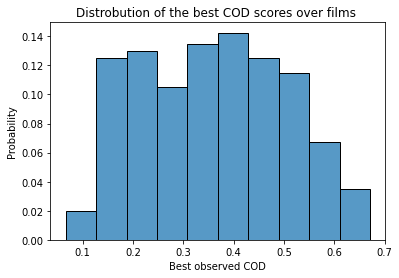
\includegraphics[width=10cm]{data anlysis project 2/figure1.png}
 \caption{}
 \label{fig:1}
\end{figure}

\begin{figure}[t]
  \centering

  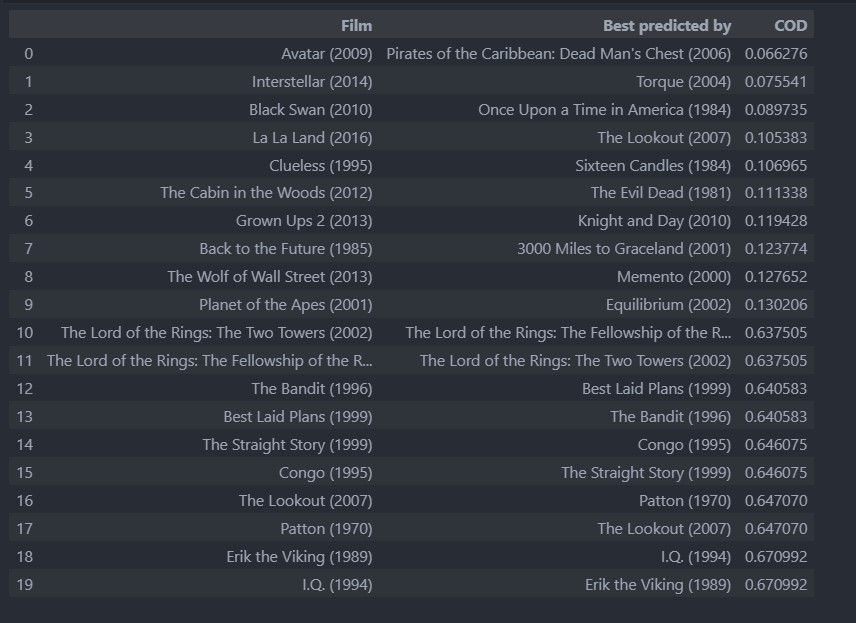
\includegraphics[width=10cm]{data anlysis project 2/apendix_figure_1.jpg}
 \caption{}
 \label{apendix fig:2}
\end{figure}

\begin{figure}[t]
  \centering

  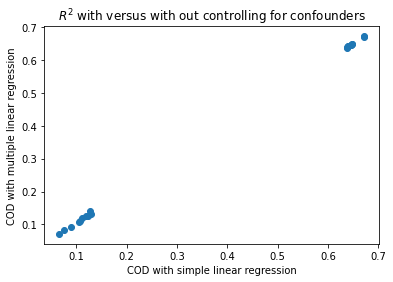
\includegraphics[width=10cm]{data anlysis project 2/figure_2.png}
 \caption{}
 \label{fig:1}
\end{figure}


\begin{figure}[t]
  \centering

  
\includegraphics[width=10cm]{data anlysis project 2/ridge_fig.jpg}
 \caption{}
 \label{fig:1}
\end{figure}
\begin{figure}[t]
  \centering

  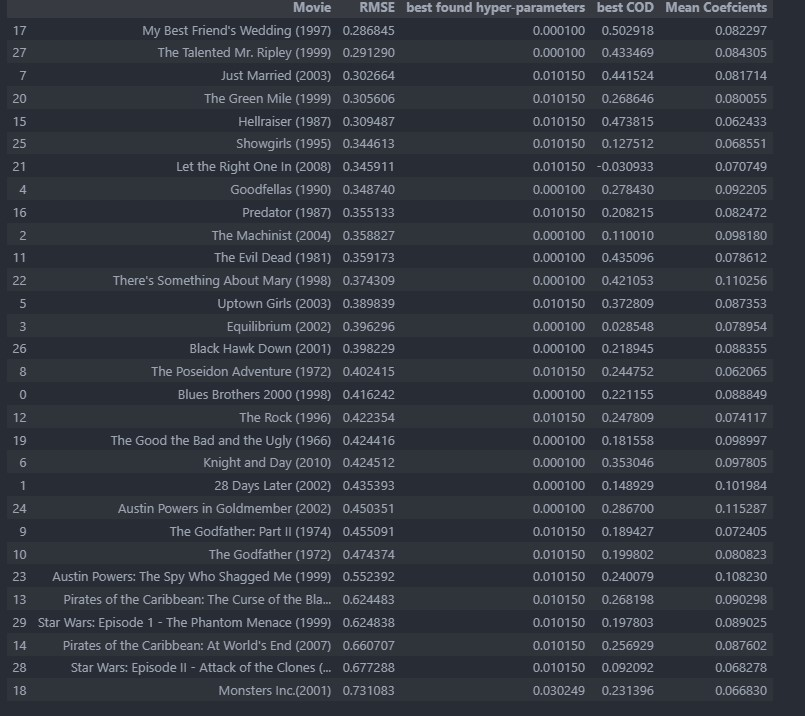
\includegraphics[width=10cm]{data anlysis project 2/lasso_fig.jpg}
 \caption{}
 \label{fig:1}
\end{figure}
\begin{figure}[t]
  \centering

  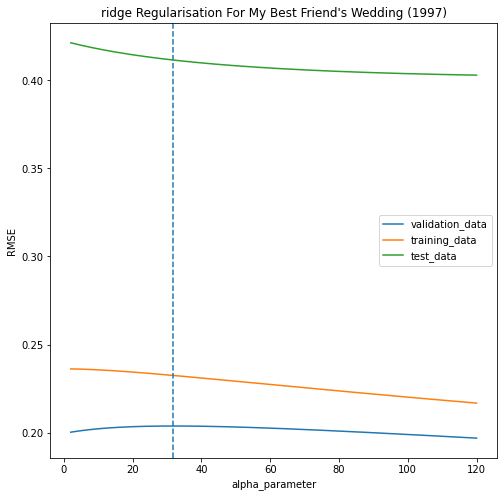
\includegraphics[width=10cm]{data anlysis project 2/fig_4.png}
 \caption{}
 \label{fig:1}
\end{figure}
\begin{figure}[t]
  \centering

  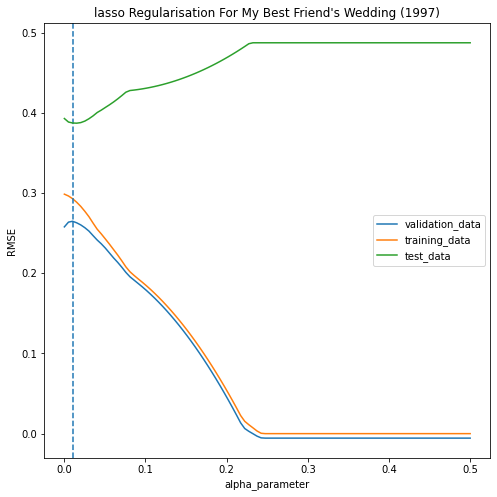
\includegraphics[width=10cm]{data anlysis project 2/fig_3.png}
 \caption{}
 \label{fig:1}
\end{figure}


\begin{figure}[t]
  \centering
  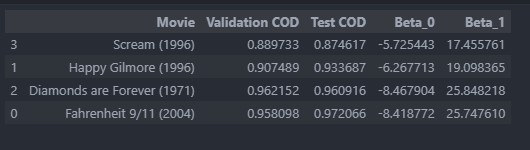
\includegraphics[width=10cm]{data anlysis project 2/question_5_1.jpg}
 \caption{}
 \label{fig:1}
\end{figure}

\begin{figure}[t]
  \centering
  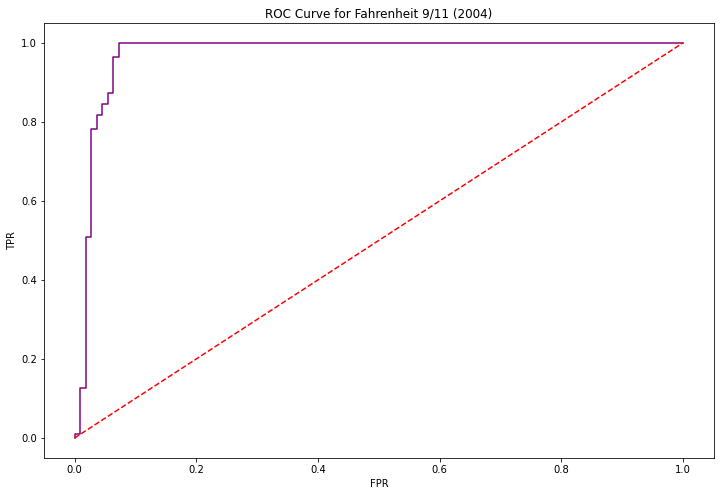
\includegraphics[width=10cm]{data anlysis project 2/logistic_1.png}
 \caption{}
 \label{fig:1}
\end{figure}

\begin{figure}[t]
  \centering
  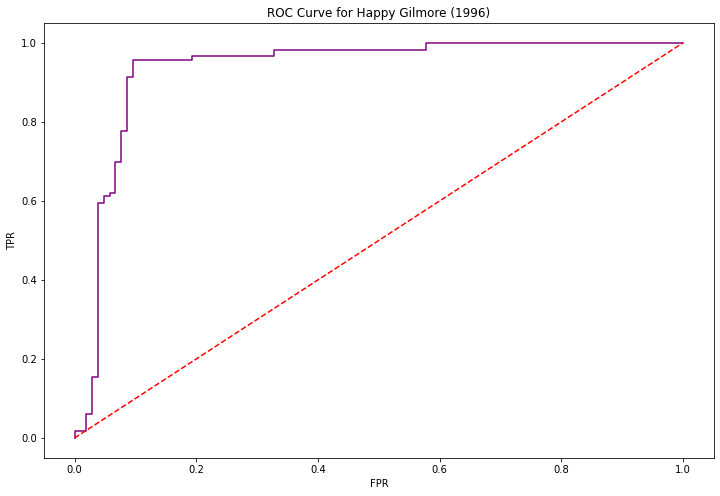
\includegraphics[width=10cm]{data anlysis project 2/logistic_2.png}
 \caption{}
 \label{fig:1}
\end{figure}

\begin{figure}[t]
  \centering
  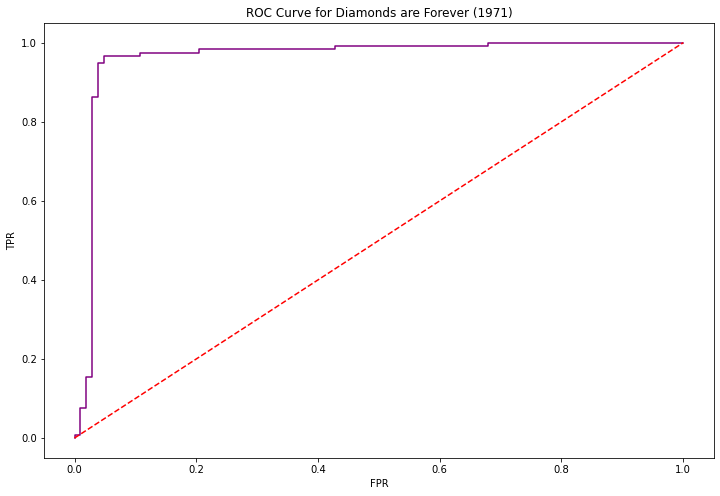
\includegraphics[width=10cm]{data anlysis project 2/logistic_3.png}
 \caption{}
 \label{fig:1}
\end{figure}

\begin{figure}[t]
  \centering
  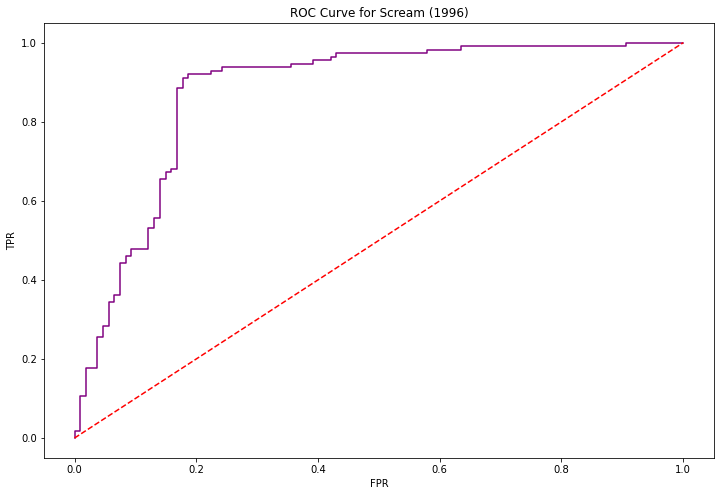
\includegraphics[width=10cm]{data anlysis project 2/logistic_4.png}
 \caption{}
 \label{fig:1}
\end{figure}

\begin{figure}[t]
  \centering
  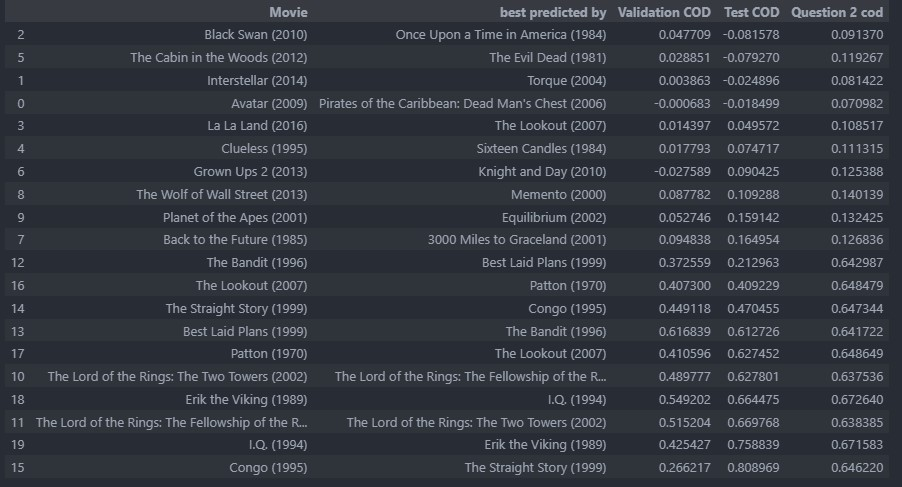
\includegraphics[width=10cm]{data anlysis project 2/extra_credit_fig.jpg}
 \caption{}
 \label{fig:1}
\end{figure}
\end{document}
